% This must be in the first 5 lines to tell arXiv to use pdfLaTeX, which is strongly recommended.
\pdfoutput=1
% In particular, the hyperref package requires pdfLaTeX in order to break URLs across lines.

\documentclass[11pt]{article}

% Change "review" to "final" to generate the final (sometimes called camera-ready) version.
% Change to "preprint" to generate a non-anonymous version with page numbers.
\usepackage[preprint]{acl}

% Standard package includes
\usepackage{times}
\usepackage{latexsym}

% For proper rendering and hyphenation of words containing Latin characters (including in bib files)
\usepackage[T1]{fontenc}
% For Vietnamese characters
% \usepackage[T5]{fontenc}
% See https://www.latex-project.org/help/documentation/encguide.pdf for other character sets

% This assumes your files are encoded as UTF8
\usepackage[utf8]{inputenc}

% This is not strictly necessary, and may be commented out,
% but it will improve the layout of the manuscript,
% and will typically save some space.
\usepackage{microtype}

% This is also not strictly necessary, and may be commented out.
% However, it will improve the aesthetics of text in
% the typewriter font.
\usepackage{inconsolata}

%Including images in your LaTeX document requires adding
%additional package(s)
\usepackage{graphicx}
\usepackage{hyperref}

% More packages and macros
\usepackage{booktabs}       % borders in tabular
\usepackage{enumitem}       % list margins
\usepackage{amssymb}        % enable \mathbb, \mathcal
\usepackage[hang,flushmargin]{footmisc}  % minimize footnote indentation
\usepackage{amsmath}
\usepackage{algpseudocode}
\usepackage{algorithm}
\usepackage[ruled,vlined]{algorithm2e}
\usepackage[english]{babel}
\usepackage[utf8]{inputenc}
\usepackage{algorithm}
\usepackage[noend]{algpseudocode}
\usepackage{hyperref}


\newcommand{\LN}{\linebreak\noindent}    % manage inline spacing
% \setenumerate[1]{leftmargin=*}    % no enumerate indentation
% \setitemize[1]{leftmargin=*}      % no itemize indentation


% If the title and author information does not fit in the area allocated, uncomment the following
%
%\setlength\titlebox{<dim>}
%
% and set <dim> to something 5cm or larger.

\title{Adapting Prompting with Haitian Creole and AAVE Using Transformer Models for Culturally and Contextually Nuanced Dialogue}

% Author Line
\author{ Ivan Martinez-Kay, Raphael Palacio \\
  Emory Univeristy Computer Science Department \\
  201 Dowman Dr., Atlanta, GA 30322 \\
  \texttt{iemarti@emory.edu} \\\
  %Affiliation / Address line 3 \\
  \texttt{raphael.palacio@emory.edu} \\}

%\author{
%  \textbf{First Author\textsuperscript{1}},
%  \textbf{Second Author\textsuperscript{1,2}},
%  \textbf{Third T. Author\textsuperscript{1}},
%  \textbf{Fourth Author\textsuperscript{1}},
%\\
%  \textbf{Fifth Author\textsuperscript{1,2}},
%  \textbf{Sixth Author\textsuperscript{1}},
%  \textbf{Seventh Author\textsuperscript{1}},
%  \textbf{Eighth Author \textsuperscript{1,2,3,4}},
%\\
%  \textbf{Ninth Author\textsuperscript{1}},
%  \textbf{Tenth Author\textsuperscript{1}},
%  \textbf{Eleventh E. Author\textsuperscript{1,2,3,4,5}},
%  \textbf{Twelfth Author\textsuperscript{1}},
%\\
%  \textbf{Thirteenth Author\textsuperscript{3}},
%  \textbf{Fourteenth F. Author\textsuperscript{2,4}},
%  \textbf{Fifteenth Author\textsuperscript{1}},
%  \textbf{Sixteenth Author\textsuperscript{1}},
%\\
%  \textbf{Seventeenth S. Author\textsuperscript{4,5}},
%  \textbf{Eighteenth Author\textsuperscript{3,4}},
%  \textbf{Nineteenth N. Author\textsuperscript{2,5}},
%  \textbf{Twentieth Author\textsuperscript{1}}
%\\
%\\
%  \textsuperscript{1}Affiliation 1,
%  \textsuperscript{2}Affiliation 2,
%  \textsuperscript{3}Affiliation 3,
%  \textsuperscript{4}Affiliation 4,
%  \textsuperscript{5}Affiliation 5
%\\
%  \small{
%    \textbf{Correspondence:} \href{mailto:email@domain}{email@domain}
%  }
%}

\begin{document}
\maketitle

\begin{abstract}
Low-resource languages and dialects such as Haitian Creole and African American Vernacular English (AAVE) often face significant challenges in natural language processing due to limited training data and complex linguistic variations. This paper introduces a novel approach combining Linguistically-Diverse Prompting (LDP), Polyglot Prompting, and conversational context tagging techniques to improve model performance across these linguistic variants. Through experiments with GPT-4o, we evaluate four model configurations that employ a combination of datasets and given techniques. Our results reveal interesting trade-offs: while simpler models excel at Natural Language Inference tasks, our more complex hybrid model demonstrates superior performance in Machine Reading Comprehension and Machine Translation. By incorporating contextual markers and poly-glottal datasets, our approach surpasses the base model's ability to handle dialectal variations while maintaining cultural sensitivity in dialogue responses. 
\end{abstract}
\section{Introduction}
\label{sec:introduction}

The use of artificial intelligence in cross-lingual settings has become more prevalent today as Large Language Models (LLMs) continue to take the world by storm. Thanks to their emergence, being able to have natural language support in a cross or multi-lingual is a reality we can enjoy. However, their still remain many under-resourced languages that are not well-supported by LLMs. We intend to further explore this area as the access to LLMs continues to expand beyond developed countries. 

Aimed to improve accessibility and user experience across low-resource languages and dialects, the improvement of translational tasks has become urgent as artificial intelligence incorporates itself into daily life. \cite{Conneau:20} introduced XLM-R, a large-scale multilingual masked language model trained on 100 languages. It demonstrates that pre-training LLMs at scale, can lead to significant performance gains for a wide range of cross-lingual transfer tasks, yet we haven't quite explored low-resource dialects and obscure languages that are not so globally spoken. Haitian Creole, to our knowledge is one such language that remains understudied by researchers working with LLMs.

Our study contributes to this expanding field by focusing on LLM performance in Haitian Creole cross-lingual tasks. Specifically leveraging datasets of African American Vernacular English (AAVE) and Standard American English as our poly-glottal and high-resource languages. 

We present a novel methodology to improve the generative and analytical capabilities of LLMs in a cross-lingual setting between SAE, AAVE and Haitian Creole using transformer-based models. Our approach centers on observing pre-trained multilingual transformer model performance with a combination dialect-specific datasets and techniques to see where trade-offs and improvements are made depending on what is combined. 

By hybridizing state of the art techniques, Linguistically-Diverse Prompting (LDP) \cite{Nguyen:24}, Polyglot Prompting \cite{Ng:22} which focus respectively on combining high-resource to low-resource languages and low-resource to low-resource languages, and contextual tags we investigate the improvement of adapting language models to Haitian Creole \cite{Upadhayay2024}. The integration of these techniques allows us to address the unique challenges presented by low-resource languages while maintaining sensitivity to their cultural and linguistic characteristics. By leveraging this methodology we show that Transformer models can effectively capture the subtle linguistic nuances that distinguish these dialects from high resource languages thus performing better in a cross-lingual setting. By enhancing the accuracy of multi-lingual identification and translation we promote greater social inclusion in language processing technologies and Artificial Intelligence in developing countries. 



\section{Related Work}
\label{sec:related-work}
                                            
\subsection{Literature Review}
Several recent studies have demonstrated significant progress in language detection; however, fewer works have focused specifically on automatic dialect detection and output. While this area remains relatively under-explored, some research has been done on related tasks.

\subsubsection{Contextual Importance}

For instance, \cite{Martin:24} highlights the integration of AI dialects to enhance user perceptions of warmth, competence, and authenticity, which in turn improves trust, satisfaction, and loyalty in AI interactions. This research emphasizes how adapting AI responses to user linguistic preferences plays a critical role in improving user engagement.

\subsubsection{Evaluating Linguistic Performance in LLMs}

And, while automatic dialect detection is not yet fully explored, benchmarks such as DIALECTBENCH \cite{Faisal:24} have introduced a large-scale NLP benchmark covering 281 varieties across 40 language clusters. This framework evaluates performance gaps between standard and non-standard dialects, promoting NLP model robustness in handling dialectal variations, especially for underrepresented languages.

Several methods have been explored to improve dialect identification and NLP performance across diverse languages and dialects. \cite{Jauhiainen:19} incorporated accent ID tokens into their model, significantly boosting performance in multi-dialect speech recognition, a technique that could also be applied to English dialects such as AAVE and Creole. Similarly, \cite{Hinsvark:21} demonstrates the effectiveness of accent ID tokens in improving model adaptability and recognition rates across a variety of accents.

In another approach, \cite{Jain:18} combined accent embeddings with multitask learning to enhance automatic speech recognition performance on accented speech, which significantly reduced error rates and improved accuracy across dialects.

\subsubsection{Prompting for Optimal Results}

Linguistically-Diverse Prompting (LDP) has recently emerged as an innovative method to enhance LLM performance, especially in low-resource languages. \cite{Nguyen:24} proposed this technique, which utilizes synthetic exemplars from high-resource languages to improve unsupervised translation, summarizing, and question answering for 34 low-resource languages. This method leverages the strong generative abilities of models like GPT-4o to improve performance across diverse linguistic tasks, including dialect identification.

Polyglot Prompting, introduced by \cite{Ng:22}, further enhances multilingual models by utilizing shared prompts across languages, improving generalization and facilitating effective cross-lingual transfer. This methodology is particularly relevant to improving dialect-specific language tasks, given the linguistic diversity of dialects such as AAVE and Creole.

Other research has explored the role of socio-cultural and cross-cultural factors in dialect identification. \cite{Garimella:16} utilized computational models like AdaBoost to identify cross-cultural differences in word usage by analyzing personal writings from the United States and Australia. The study used classifiers based on linguistic features and topic modeling to uncover how language reflects cultural biases, enhancing dialect detection through cultural awareness.

Additionally, integrating external knowledge sources can further improve NLP models. \cite{Camboim:24} proposed using Knowledge Graphs (KGs) alongside LLMs to enhance chatbots' ability to understand socio-cultural contexts during user interactions, specifically in the context of machine translation. This combination of KGs and LLMs enhances the model's capacity to capture cultural intricacies, improving translation accuracy and contextual understanding in dialects.

Finally, \cite{Goldin:18} explored Native Language Identification (NLI), combining linguistically motivated features with social network characteristics to improve the accuracy of distinguishing between native and non-native speakers. This method leveraged linguistic patterns and user behavior on platforms like Reddit to capture subtle differences in language use across speakers' native languages, contributing to improved dialect recognition.

\subsubsection{Data}

The availability of high-quality data is essential for improving NLP models, especially for dialect-specific tasks. \cite{Lent:24} introduced CreoleVal, a multilingual benchmark that spans 28 Creole languages and covers various NLP tasks such as reading comprehension, relation classification, and machine translation. By curating novel datasets and applying transfer learning from higher-resourced ancestor languages, this study enhanced NLP model performance for Creole languages. Importantly, it emphasizes the need for cultural sensitivity in language processing, which is critical for dialect adaptation and recognition, meaning our search for contextual nuance in datasets was key to our model function.

\cite{Upadhayay2024} demonstrate TaCo (translation-assisted chain-of-thought) reasoning which enhances cross-lingual transfer in datasets for low-resource languages, achieving significant improvements in multilingual LLM performance across several low-resource languages. The Haitian Creole dataset we use in our study is also their creation. In their study, they did not make use of the Haitian Creole dataset. 

Our SAE dataset hails from \cite{kim2022} PROSOCIALDIALOG which introduces the first large-scale multi-turn dialogue dataset designed to guide conversational agents in responding to potentially unsafe user inputs following prosocial norms. The dataset includes 58,000 dialogues, 331,000 utterances, 160,000 unique rules-of-thumb, and 497,000 safety labels with rationales. Matching our interests in contextual dialogue, this dataset provides an excellent high-resource language pool, that can easily be mapped to our chosen low-resource language.

 The Corpus of Regional African American Language (CORAAL) \cite{kendall23} presented a corpus of untagged AAVE dialogue, which complements our use of polyglottal languages. Additionally, CORAAL offers a comprehensive and regionally diverse collection of African American Vernacular English (AAVE) data. The latest CORAAL version (2023.06) includes over 220 speakers, notably incorporating a new Detroit 1966 dataset with 40 speakers from the classic Detroit Dialect Study. This resource aligns well with our study's goals of exploring linguistic diversity and dialectal nuances in natural language processing tasks.

\subsubsection{Challenges}

Many existing models still face challenges when distinguishing between closely related dialects, particularly in low-resource languages such as AAVE and Creole. For example, while \cite{Jauhiainen:19} successfully integrated accent ID tokens to improve multi-dialect recognition, their approach struggled with highly similar dialects that have subtle phonetic differences, such as AAVE and SAE. This suggests utilizing ID tokens in our hybrid model might complicate the cross-lingual tasks between SAE and AAVE. 

Benchmarks like DIALECTBENCH \cite{Faisal:24}, though comprehensive in covering a wide variety of languages, reveal that performance gaps still exist between standard and non-standard dialects. The underrepresentation of dialect-specific data in these benchmarks poses a significant challenge, as models tend to over-fit to high-resource languages and struggle with the dialects that fall outside this scope. DIALECTBENCH currently has only been tested with mBERT, XLM-r, and NLLB. Adapting it to benchmark GPT-4o may prove to be another limitation, possibly leading to inconsistencies in our evaluation results.

Furthermore, approaches like Linguistically-Diverse Prompting (LDP) \cite{Nguyen:24} have demonstrated success in improving performance for low-resource languages, yet they still depend heavily on the availability of high-quality exemplars from related high-resource languages. This creates a limitation when there is insufficient data for the source or target languages, leading to diminished model performance, especially in cases where dialects do not have an extensive linguistic corpus.

While \cite{Lent:24} introduces CreoleVal to address the gap in data for Creole languages, it highlights a broader issue in dialect-specific NLP: the scarcity of large, annotated datasets which we only found in SAE.
\section{Approach}
\label{sec:approach}

Our approach builds off of state-of-the-art techniques Linguistically Diverse Prompting (LDP) \cite{Nguyen:24} and Polyglot Prompting (PolyP) \cite{Ng:22} that have improved LLM cross-lingual performance previously. By incorporating cultural and conversational context tags to our datasets, we can further improve the model's performance and target linguistic adaptation for better conversation. While we are currently only working and applying our prompting techniques to a limited number of datasets, we believe this methodology can be universally adapted to other language combinations. Lastly by utilizing DIALECTBENCH \cite{Faisal:24} on the initial model schemas and then our hybridized model, we get an idea of the LLM's improvement in these lower-resource languages in a cross-lingual setting.

\subsection{Cultural and Contextual Inclusion}

For each document \(x_j \in D_X\), where \(D_X\) is a dataset of the target low-resource language \(X\), we augment the input with a cultural and contextual tag. This tag, denoted as \(c_j\), encodes conversational context (casual and formal) and cultural markers (urban, rural, and specific linguistic features). The input sentence \(x_j\) is thus represented as:

\[
x_j = (w_j, c_j)
\]

\noindent We let:

\begin{itemize}
    \item \(w_j\) denote the tokenized words of the sentence.
    \item \(f_j\) denote formal speech.
    \item \(t_j\) denote casual speech.
    \item \(u_j\) denote urban speech.
    \item \(r_j\) denote rural speech.
    \item \(lf_j\) denote linguistic features specific to the language or dialect.
\end{itemize}

Thus, the cultural context \(c_j\) is defined as:

\[
c_j \in \{f_j, t_j\} \times \{u_j, r_j, lf_j\}
\]

This representation of \(c_j\) allows the model to incorporate both conversational and cultural markers, improving its understanding of the context in which a sentence is used.

In the case of polyglot prompting \cite{Ng:22}, we extend this approach by including multiple languages in the exemplar set \(Z_i\). For each text sample, we construct prompts from multiple high-resource languages \(Z_i \in \text{High-Resource Languages}\), incorporating the same cultural and contextual markers \(c_{zi}\) as follows:

\[
\small
E_{Z_i} = \{(z_i, c_{zi}, e_{zi}) \mid Z_i \in \text{High-Resource Languages}\}
\]

\begin{itemize}
    \item \(z_i\) is a sample document from the high-resource language \(Z_i\).
    \item \(e_{zi}\) is the corresponding English translation.
    \item \(c_{zi}\) encodes the cultural and contextual markers for each exemplar.
\end{itemize}


For an input document \(x_j\) from a low-resource language, the model detects the cultural context \(c_j\) and uses the polyglot exemplars to better understand how to translate or respond \cite{Ng:22}. The translation task is formalized as:

\[
\small
F_{\text{X} \to \text{E}}(x_j, c_j) = \mathbb{P}(e_j \mid x_j, c_j, z_1, e_{z_1}, \dots, z_n, e_{z_n})
\]

\begin{itemize}
    \item \(e_j\) is the output.
    \item \(z_i\) and \(e_{z_i}\) are the high-resource language exemplars guiding the model.
\end{itemize}

\subsection{Cultural and Contextual Detection}

To facilitate cross-lingual tasks \cite{Nguyen:24}, we gather exemplar pairs from high-resource languages \(Z_i \in \text{High-Resource Languages}\). Each exemplar pair includes cultural and contextual tags \(c_{zi}\) alongside the linguistic features. This is formalized as:

\[
\small
E_{Z_i} = \{(z_i, c_{zi}, e_{zi}) \mid Z_i \in \text{High-Resource Languages}\}
\]

For an input sentence \(x_j\) from a low-resource language, the model detects the cultural context \(c_j\) and uses the exemplars from high-resource languages to better understand how to translate or respond \cite{Nguyen:24}. The process is formalized as:

\[
\small
F_{\text{X} \to \text{E}}(x_j, c_j) = \mathbb{P}(e_j \mid x_j, c_j, z_1, e_{z_1}, \dots, z_n, e_{z_n})
\]

Where \(e_j\) is the output (dialogue response and analysis) and \(z_i\) are the exemplars guiding the model.

\subsection{Adapting to Dialects}

The final objective is for the model to automatically adapt to the dialect and conversational style of the input without needing explicit prompting. Given an input \(x_j\) with contextual markers \(c_j\), the model generates a response \(re_j\) in the same dialect that can then be evaluated through DIALECTBENCH \cite{Faisal:24}, formalized as:

\[
\small
F_{\text{Adapting}}(x_j, c_j) = \mathbb{P}(re_j \mid x_j, c_j, z_1, e_{z_1}, \dots, z_n, e_{z_n})
\]

\subsubsection{Defining The Input and Prompts}

\[
\text{Datasets} = \{D_1, D_2, D_3\}
\]

\begin{itemize}
    \item \(D_o \in \{\text{AAVE, Haitian Creole}\}\) alternates between AAVE and Haitian Creole for fine-tuning. such that $D_1 \neq D_2$ and $D_1, D_2 \in D_o$.
    \item \(D_1 \) serves as the low-resource language being bench-marked and translated.
    \item \(D_2 = \text{English dataset}\).
    \item \(D_3\) serves as the additional polyglot language.
\end{itemize}

\textbf{Prompt} is defined as:
\begin{itemize}
    \item Cultural and contextual analysis flag (formal / casual, urban / rural, and linguistic characteristics).
    \item Use of LDP and PolyP techniques for cross-lingual understanding.
\end{itemize}

\subsubsection{Hybrid Model Prompt}\\
\begin{enumerate}
    \item Observe the linguistic features in \{\textbf{D2}\} (since you are extensively trained in English).
    \item Translate the content of each \{\textbf{D1}\} entry into the language or dialect used in its corresponding \{\textbf{D2}\} entry.
    \item Conduct a translation task where you translate the dialect in \{\textbf{D1}\} to the dialect/language in \{\textbf{D3}\}.
    \item Perform a cultural and conversational context analysis of \{\textbf{D1}\} based on the shared similarities with \{\textbf{D2}\} and \{\textbf{D3}\}.
    \item Detect and report contexts.
    \item Reprompt yourself with the same tasks using the language spoken in \{\textbf{D1}\}, then reprompt yourself with the same tasks by translating the reprompt in \{\textbf{D1}\} with the language spoken in \{\textbf{D3}\}.
    \item Provide a dialogue response in language \{\textbf{D1}\} (Haitian Creole) or a continuation based on what the speaker said in language \{\textbf{D2}\} (English) and \{\textbf{D3}\} (AAVE), respectively.
\end{enumerate}\\

\subsubsection{Simultaneous Feeding}

All data sets \(D_1, D_2,\) and \(D_3\) are fed into the API along with the cultural and contextual analysis tags and prompts:

\begin{figure}[H]
    \centering
    \includegraphics[width=1\linewidth]{Screenshot 2024-12-13 at 10.32.32 PM.png}
    \label{fig:enter-label}
\end{figure}


\subsection{LDP (Linguistic-Diverse Prompting)}
Linguistically-Diverse Prompting (LDP) has recently emerged as a robust approach to adapting language models, especially in tasks dealing with low-resource dialects such as AAVE and Creole. LDP uses examples from high-resource languages to improve low-resource language tasks by transferring linguistic structures and patterns. This method enables models to learn related languages or dialects and apply that learning to dialects with limited training data. For example, \cite{Nguyen:24} demonstrated how LDP can use synthetic exemplars from high-resource languages to enhance unsupervised tasks such as translation, summarization, and answering questions for low-resource languages.

LDP supports few-shot learning, a technique that allows models to generalize from minimal labeled data, which is crucial for dialects where large-scale datasets are often unavailable. The strong generative abilities of models like GPT-4o make LDP particularly effective in improving the adaptation and detection of dialects. By fine-tuning LDP on small dialect-specific datasets, it is possible to better capture unique linguistic features, such as phonetic and syntactic variations inherent in dialects like AAVE or Creole.

\subsubsection{Why LDP?} 
LDP provides a way to improve dialect detection and language generation by helping models adapt to low resource languages and dialects that are underrepresented in traditional datasets. The ability of LDP to handle cross-lingual tasks with minimal data makes it a valuable method to refine the ability of our model to detect and respond to AAVE and Creole. Our model can capture nuanced linguistic features specific to our data without requiring varied corpora, which are often unavailable. Thus, incorporating LDP would enhance both the accuracy and cultural sensitivity of the model, making it's cross-lingual generation more nuanced.

\subsection{Polyglot Prompting}
Polyglot Prompting is another method that improves multilingual and multi-dialectal language tasks by utilizing prompts in multiple languages or dialects. This technique allows large language models to dynamically adapt to various linguistic contexts. For instance, \cite{Ng:22} demonstrated how Polyglot Prompting enhances model generalization across different languages by leveraging shared linguistic structures and facilitating cross-lingual transfer.

By using polyglot prompts, models can learn to respond appropriately in multiple dialects, improving linguistic flexibility. This approach is particularly relevant for AAVE and Haitian Creole, as these dialects often involve code-switching or dialectal shifts in real-world language use. Polyglot prompting enables the model to recognize and respond based on the dominant dialect in the user’s input, ensuring a contextually appropriate response.

\subsubsection{Why Polyglot Prompting?}
Polyglot Prompting helps ensure that our model can dynamically respond to various English dialects. By exposing the model to prompts in Haitian Creole we can adapt it seamlessly to dialectal shifts in real-time conversations. This will significantly improve the model’s ability to handle multilingual environments or situations where users frequently switch between dialects. In essence, Polyglot Prompting supports our goal of building a model that is flexible and responsive to diverse linguistic inputs.
\section{Experiments}
\label{sec:experiments}

\subsection{Data}

\subsubsection{Data Tagging}

In order to enhance the linguistic adaptability of our model across different dialects and languages, we conducted a detailed data tagging process using the BGE (Bilingual Generalized Embedding) model. The BGE model allowed us to generate embeddings for each data entry, which were then compared to predefined tags, enabling us to assign contextually relevant linguistic features to our dataset. This tagging process was essential for building a robust dataset that accurately reflects the stylistic and grammatical differences present in each dialect.

\textbf{Tagging Process}: Each text entry in our dataset was embedded using the BGE model's embeddings. The embeddings were generated based on a set of linguistic parameters, including dialect, setting, tone, and linguistic features. These categories were defined as follows:
\begin{itemize}
    \item \textbf{Dialect}: Tags for different dialects such as AAVE (African American Vernacular English), Haitian Creole, and SAE (Standard American English) were used to represent the dominant linguistic style of each entry.
    \item \textbf{Setting}: This parameter categorized entries as either \textit{urban} or \textit{rural} based on the contextual setting inferred from the text.
    \item \textbf{Tone}: Entries were classified with either a \textit{formal} or \textit{informal} tone to capture variations in grammatical structure and word choice.
    \item \textbf{Linguistic Features}: Specific linguistic features, such as phonetic contractions (e.g., “gonna” or “ain’t”) and French-derived lexicon in Haitian Creole, were tagged to provide additional contextual cues for the model during training and evaluation.
\end{itemize}

\textbf{Parameter Settings}: For each tag example (such as "urban," "formal," or "AAVE"), we generated embeddings using the BGE model. The embeddings were derived with a maximum token length of 512, which ensured each text entry was adequately represented without truncation. We applied cosine similarity between each entry’s embedding and the predefined tag embeddings to determine the closest matching tag. The highest similarity score within each category was selected as the final tag for that category, thus providing a multi-dimensional linguistic characterization of each entry.

This tagging process allowed us to annotate each text with comprehensive linguistic metadata, which facilitated improved performance during model training. It also enabled us to evaluate the model’s ability to adapt to diverse dialects and linguistic features, a critical requirement for assessing dialectal and linguistic accuracy in our evaluation stage.


\subsubsection{AAVE Dataset}
The African American Vernacular English (AAVE) dataset used in this study is derived from the CORAAL project \cite{kendall23}, specifically from the Atlanta section of the corpus. The dataset consists of dialogues representing natural spoken AAVE, collected from interviews and other conversational contexts. Each entry in the dataset includes fields for the speaker, start time, content, and end time of each utterance. The content covers a wide range of informal dialogue, reflecting cultural and linguistic nuances specific to the AAVE dialect.

Following best practices for dataset preparation, we divided the AAVE data into training, development, and test sets using an 80/10/10 split ratio. This split ensures a representative distribution of linguistic features across the three sets while allowing for effective model evaluation. The split is outlined in Table~\ref{table:aave-split}.

\begin{table}[h]
    \centering
    \begin{tabular}{|l|c|c|c|}
        \hline
        \textbf{Set} & \textbf{Dialogues} & \textbf{Length} & \textbf{Tags} \\
        \hline
        Training & 19,080 & 461,267 & 76,320 \\
        Development & 2,385 & 56,881 & 9,540 \\
        Test & 2,386 & 58,737 & 9,544 \\
        \hline
    \end{tabular}
    \caption{Data split for AAVE dataset. The "Length" column refers to the total length of dialogues in tokens, and "Tags" refers to linguistic annotations associated with each entry.}
    \label{table:aave-split}
\end{table}

\subsubsection{Haitian Creole Dataset}
The Haitian Creole dataset used in this research is adapted from the Alpaca Haitian Creole Taco dataset \cite{SAILLab:24}, a collection of prompts and responses designed to train conversational models in the Haitian Creole language. Each entry in the dataset includes an "Instruction" (task prompt), "Input" (optional additional context), and "Output" (expected response). The dataset reflects formal and informal tones and covers vocabulary specific to Haitian Creole.

Following a similar approach to the AAVE dataset, we split the Haitian Creole dataset into training, development, and test sets with an 80/10/10 ratio. The split ensures coverage of different linguistic and contextual markers for reliable evaluation. Table 2 presents the split distribution.

\begin{table}[h]
    \centering
    \small  % Reduces the font size of the table
    \setlength{\tabcolsep}{4pt} % Adjusts the space between columns
    \renewcommand{\arraystretch}{1.1} % Adjusts row height for compactness
    \begin{tabular}{|c|c|c|c|}
    \hline
    \textbf{Set} & \textbf{Dialogues} & \textbf{Instruction Length} & \textbf{Tags} \\
    \hline
    Training & 39,680 & 2,175,336 & 158,720 \\
    Development & 4,960 & 273,196 & 19,840 \\
    Test & 4,961 & 271,184 & 19,844 \\
    \hline
    \end{tabular}
    \caption{Data split for Haitian Creole dataset. The "Instruction Length" column denotes the total token length for instructions, and "Tags" refers to linguistic annotations assigned to each entry.}
\end{table}

\subsection{Data Split Rationale}
To ensure a balanced and effective distribution of linguistic features across all subsets, we followed established best practices in data splitting. For datasets with more than 10,000 instances, an 80/10/10 split was applied, where 80\% of the data was reserved for training, 10\% for development, and the remaining 10\% for testing. This approach allows for robust training and reliable validation and testing phases, providing comprehensive evaluation metrics for each dialect. Cross-validation techniques were considered but deemed unnecessary given the large size of both datasets.

\subsection{Experimental Settings}

Our experiments were conducted on Google Colab's high-performance computational platform, utilizing the cloud's high ram CPUs, which allowed us to efficiently iterate over the data splits for our experiments. All models were given a max token generation parameter of 2500 and by reading in the data by batches (Batch size of 5) and adding multiple entries per input tag, we streamlined the models' data reading process for a broader analysis across a larger dialogue. Not only does this make the processing faster, but it provides a broader conversational context that the model recognizes. In this specific iteration of experiments we define $D_1$ = Haitian Creole, $D_2$ = Standard American English, and $D_3$ = African American Vernicular English.

We gave the base model a temperature of $0.5$ to encourage some exploration in the dataset without losing logical functionality. The LDP and PolyP models were ran at a slightly higher temperature of $0.6$ to encourage further delving into dialectal tags and intricacies. Since both these models were provided with more data, we believe the larger context might mitigate for loss of reasoning. Finally our hybrid model that was provided with all three tagged datasets, was given the most freedom to explore with a temperature of $0.7$. 

\textbf{Dialect-Specific Prompting:} Through LDP, the model was prompted with exemplar prompts that encouraged dialect-specific adaptation for Haitian Creole. This included the usage of sample dialogues reflecting common phraseology in both AAVE and SAE. Polyglot prompting was introduced to facilitate real-time language adaptation, allowing the model to handle code-switching between our low resource languages and dialects.

\subsection{Model Development}

\subsubsection{LLaMA Model Development}

\textbf{Model Configuration and Initialization:} We initially wanted to run our experiments with a base Llama 3.2, but discovered that it has no prior knowledge of Haitian Creole speech. We omitted this model to focus on our GPT-4o implementations.

\textbf{Training Objectives and Fine-tuning Strategy:} Given the domain-specific focus on AAVE and Haitian Creole, we wanted to fine-tune using domain-specific prompts under Linguistically-Diverse Prompting (LDP) and Polyglot Prompting methods. The training data was curated to cover various linguistic and contextual features, such as informal, formal, urban, and rural tones. During fine-tuning, we wanted to emphasize dialect-sensitive response generation, adjusting the model’s attention layers to adapt dynamically to dialect-specific syntactic and lexical patterns. We planned to incorporate a test run with a fine-tuned model using LLaMA 3.2. LLaMA 3.2 is not previously trained in our chosen low-resource languages, so this meant that we would have needed to train it in said low-resource languages, unlike GPT-4o that might not be fine-tuned, but is still trained.

\subsubsection{GPT-4o}

\textbf{Model Configuration and Use Case:} For the GPT-4o model, we used OpenAI’s API without any additional fine-tuning, taking advantage of its pre-existing capabilities in handling diverse language structures and dialects. GPT-4o's architecture, pretrained on a broad array of multilingual and multidialectal data, allows it to generalize effectively to tasks involving AAVE, Haitian Creole, and SAE without requiring additional training on specific dialectal datasets.

\textbf{Inference Strategy:} Instead of fine-tuning, we leveraged GPT-4o in a zero-shot or few-shot configuration. This involved designing prompts to instruct GPT-4o to recognize and respond in the appropriate dialect based on contextual and linguistic cues. For instance, prompts were structured to inform GPT-4o to generate responses that mirror the syntactic and lexical norms of AAVE or Haitian Creole, as well as to switch between dialects as needed. Linguistically-Diverse Prompting (LDP) and Polyglot Prompting techniques were employed in the prompts to maximize dialectal adaptation.


\textbf{Evaluation of GPT-4o’s Dialect Adaptation:} Although not fine-tuned, GPT-4o’s outputs were evaluated on dialect-specific F1 score metrics provided by DialectBench \cite{Faisal:24} to assess its effectiveness in generating responses that align with AAVE and Haitian Creole linguistic norms. DialectBench was employed to measure F1 scores on dialectal NLP tasks.

\subsection{Evaluation Metrics}

To assess the performance of our model in handling dialectal variations, we employ DialectBench \cite{Faisal:24}, a comprehensive benchmarking framework designed for evaluating dialectal and linguistic accuracy across NLP tasks involving closely related languages and dialects \cite{Faisal:24}. DialectBench provides a systematic approach to evaluating language models on non-standard dialects by measuring their ability to accurately generate and respond with dialect-specific linguistic features. The following relevant tasks were measured: Natural Language Inference (NLI), Machine Reading Comprehension (MRC), and Machine Translation (MT).

\subsubsection{DIALECTBENCH}
DIALECTBENCH \cite{Faisal:24} uses the F1 score as a core evaluation metric to capture a balanced measure of precision and recall in the detection and generation of dialect responses. The F1 score is particularly well-suited for tasks requiring dialectal adaptation, as it enables us to quantify how effectively the model can distinguish and reproduce unique linguistic characteristics associated with different dialects, such as syntax, and lexicon. 

In our experiments, the F1 score is calculated based on the precision of the model to respond to inputs in AAVE (African American Vernacular English) and Haitian Creole, comparing these outputs to expected responses that adhere to dialect-specific features. By fine-tuning the model in each dialect, our aim is to improve the F1 scores by aligning the model output with relevant linguistic markers for each variety.

We made use of DIALECTBENCH's machine translation) scoring system. BLEU serves as a fundamental metric in machine translation evaluation, calculating similarity scores between machine-generated translations and reference human translations found in $D_1, D_2$ and $D_3$. The scoring system we utilized operates by comparing n-grams (sequences of consecutive words) between the candidate and reference translations, typically evaluating sequences from uni-grams to 4-grams.

Our adapted DIALECTBENCH \cite{Faisal:24} metric \textbf{Natural Language Inference (NLI)} involved premises and hypotheses derived from AAVE and Haitian Creole datasets. These were selected based on our chosen cultural and contextual tags. We assigned GPT-4o to annotate ground truth labels for entailment, contradiction, or neutral relationships in our generated responses and data. 

The subsequent metric \textbf{Machine Reading Comprehension (MRC)} compared paragraphs selected from AAVE and Haitian Creole datasets and corresponding analysis generated by our models. F1 scores evaluated token-level matches between predictions and ground truth, emphasizing the inclusion of contextual markers (\(c_j\)) in comprehension tasks.

\[
\small
F_1 = 2 \cdot \frac{\text{Precision} \cdot \text{Recall}}{\text{Precision} + \text{Recall}}
\]

\textbf{Machine Translation (MT)} utilized BLEU scores (\(\text{Bilingual Evaluation Understudy}\)) to evaluate the final generated dialogue responses $r_{ej}$.
\[
\small
\text{BLEU} = \exp\left(\min\left(1 - \frac{l_{r_{e_j}}}{l_{e_{z_i}}}, 0\right) + \sum_{n=1}^N w_n \log p_n \right)
\]

where \(l_{r_{e_j}}\) is the candidate translation length, \(l_{e_{z_i}}
\) is the reference length, \(p_n\) is the precision for n-grams, and \(w_n\) are weights for n-gram precision.\\ 


\subsection{Results}
\begin{table}[H]
\centering
\begin{tabular}{|l|c|c|}
\hline
\textbf{Model} & \textbf{NLI (F1)} & \textbf{MRC (F1)} \\ \hline
Base Model & 0.645 $\pm $ 0.106 & 0.803 $\pm $ 0.065 \\ \hline
LDP Model & 0.617 $\pm $ 0.085 & 0.755 $\pm $ 0.098\\ \hline
PolyP & 0.595 $\pm $ 0.093 & 0.903 $\pm $ 0.056 \\ \hline
Combo Model & 0.561 $\pm $ 0.081 & 0.924 $\pm $ 0.042 \\ \hline
\end{tabular}
\caption{Natural Language Inference and Machine Reading Comprehension Performance}
\label{tab:model-performance}
\end{table}

\begin{table}[H]
\centering
\begin{tabular}{|l|c|}
\hline
\textbf{Model} & \textbf{MT BLEU Score} \\ \hline

Base Model & 2.456 $\pm $ 3.359 \\ \hline
LDP Model & 3.804 $\pm $ 4.009\\ \hline
PolyP Model & 6.507$\pm $ 8.866 \\ \hline
Combo Model & 18.057 $\pm $ 10.703\\ \hline

\end{tabular}
\caption{Machine Translation Performance}
\label{tab:mt-bleu-performance}
\end{table}

\subsection{Interpretation}

The results presented in tables~\ref{tab:model-performance} and~\ref{tab:mt-bleu-performance} reveal important insights into the performance of various language models across different tasks. Key findings indicate that the more complex Hybrid and PolyP models generally outperform the LDP and base models in translation tasks, particularly when contextual tags and polyglot datasets are provided. 

There is an inverse relationship between model complexity and Natural Language Inference (NLI) performance, where simpler models actually outperform their more complex counterparts. As noted in Figure~\hyperref[fig:nli-scores]{3} the Base Model achieves the highest F1 score of 0.645, while the more sophisticated Hybrid Model shows the lowest at 0.561. However, this pattern is completely in table Figure~\hyperref[fig:mrc-scores]{4}, where the Hybrid Model excels with an impressive F1 score of 0.924 compared to the Base Model's 0.803. Furthermore we see an even more dramatic difference in table Figure~\hyperref[fig:mt-scores]{5}, where the Hybrid Model achieves a BLEU score of 18.057, vastly outperforming the Base Model's score of 2.456.

These results suggest important implications about the relationship between model complexity and task-specific performance. While increased model complexity and a higher temperature appears to benefit both MRC and MT tasks substantially, it seems to interfere with NLI capabilities. This could indicate potential task interference in multi-task learning scenarios or suggest that different language understanding tasks may require different architectural approaches. The stability of performance also varies significantly across tasks. MRC shows relatively consistent improvements with smaller standard deviations, while MT exhibits high variance in performance, with standard deviations exceeding the magnitude of the scores themselves.

The findings raise several critical questions for future research. First, the consistent degradation in NLI performance across more complex models warrants investigation, as it challenges the common misconception that more sophisticated models necessarily perform better. Second, the high variance in MT scores suggests the need for re-evaluation on our tagging approach. This may also indicate a need for further studies in other low-resource languages where cross-lingual tasks are not as extreme.






\section{Analysis}
\label{sec:analysis}

\subsection{Model Performance}

In our experiments, we ran four models in sequence to find a trend in performance. This section presents a discussion and evaluation of the four models: Base Model, LDP Model, PolyP Model, and Hybrid Model across three of  DIALECTBENCH's \cite{Faisal:24} tasks: Natural Language Inference (NLI), Machine Reading Comprehension (MRC), and Machine Translation (MT). 

\subsubsection{Natural Language Inference (NLI)}

The results in Table~\ref{tab:model-performance} show that the \textbf{Base Model} achieves the highest NLI F1 score (\(0.645 \pm 0.106\)), suggesting a stronger generalization in inferring logical relationships in cross-lingual dialogue. Compared to the Base Model, the inclusion of linguistic diversity in the \textbf{LDP Model} results (0.617 $\pm $ 0.085) in a performance drop of approximately \(4.34\%\), indicating potential noise introduced by the inclusion of a high-resource language and contextual markers in the prompts.

The \textbf{PolyP Model} (\(0.595 \pm 0.093\)) demonstrates a further performance decline of approximately \(7.75\%\) relative to the Base Model, likely due to increased complexity in balancing multilingual exemplars and dialectal features. The \textbf{Hybrid Model} (\(0.561 \pm 0.081\)) experiences the largest drop of approximately \(13.02\%\) compared to the Base Model, suggesting that combining techniques may lead to overcompensation to specific dialectal and contextual features.


\subsubsection{Machine Reading Comprehension (MRC)}

The results in Table~\ref{tab:model-performance} show that the \textbf{Hybrid Model} achieves the highest MRC F1 score (\(0.924 \pm 0.042\)), demonstrating that a combined approach of Linguistically Diverse Prompting (LDP) and Polyglot Prompting (PolyP) enhances the model's understanding of nuanced textual information in a cross-lingual context. The \textbf{PolyP Model} (\(0.903 \pm 0.056\)) also performs well, leveraging multilingual exemplars for improved comprehension.

The \textbf{Base Model} (\(0.803 \pm 0.065\)) performs reasonably well but lacks the contextual depth provided by cultural and conversational markers. Interestingly the \textbf{LDP Model} (\(0.755 \pm 0.098\)) under-performs relative to the Base Model. This suggests that combining contextual markers (\(c_j\)) with multilingual exemplars significantly improves comprehension tasks in most scenarios, and that utilizing a high resource language (SAE) in this particular case doesn't improve the model's comprehension in a cross-lingual setting. With an increase in score by more than $10\%$ the \textbf{PolyP Model} and \textbf{Hybrid Model} results suggest that polyglot prompting might significantly improve the model's comprehension with our low resource language (Haitian Creole) with further contextual enhancement found in the \textbf{Hybrid Model}'s prompting style also improving performance. 

\subsubsection{Machine Translation (MT)}

Table~\ref{tab:mt-bleu-performance} shows that the \textbf{Hybrid Model} achieves the highest BLEU score (\(18.057 \pm 10.703\)) followed by the \textbf{PolyP Model} (\(6.507 \pm 8.866\)). Though these scores are all far below average, the \textbf{Hybrid Model} performs roughly 2.775 times better than it's runner-up. This suggests that the inclusion of $D_1$ (Main Dialect/Language), $D_2$ (High Resource Language), and a $D_3$ (Polyglottal Language) with contextual markers might significantly improve a model's cross-lingual translational ability.

The \textbf{LDP Model} (\(3.804 \pm 4.009\)) shows minimal improvement over the \textbf{Base Model} (\(2.456 \pm 3.359\)), indicating that linguistic diversity positively impacts translation tasks. However, the results suggest that the combination of LDP and PolyP techniques, as employed in the Hybrid Model, is crucial for achieving higher-quality translations in low-resource languages.

\subsubsection{Trends}

Across all tasks, a clear trade-off emerges between model complexity and task-specific performance. The \textbf{Base Model} excels in NLI tasks, where logical consistency and simplicity are critical. In contrast, the \textbf{Hybrid Model} consistently outperforms others in MRC and MT tasks, demonstrating the effectiveness of integrating cultural and contextual markers (\(c_j\)) with multilingual exemplars (\(z_i, e_{z_i}\)). This is highlighted in Figure 5 where the trade-off is presented in a steep slope seen in the third evaluation run.

The decline in NLI performance for LDP and PolyP models highlights the difficulty of balancing linguistic diversity with logical inference. In contrast, the gains in MRC and MT tasks underscore the importance of cultural and conversational adaptation, which enhances the model's understanding and generation capabilities across dialects and languages.

\subsection{Error Analysis}
Our evaluation of the Base, LDP, PolyP (Polyglot Prompting), and Hybrid (LDP + Polyglot) models highlights distinct patterns in errors, closely aligned with the performance trends discussed earlier. These patterns reflect the interplay between linguistic diversity, dialect-specific adaptability, and cultural nuances across tasks. Below, we provide a detailed breakdown of error types observed across models.

\subsubsection{Task-Specific Performance}
While the \textbf{Base Model} excelled in Natural Language Inference (NLI), its performance dropped significantly in Machine Reading Comprehension (MRC) and Machine Translation (MT). This suggests that simple prompting style with minimal contextual inclusion are beneficial for logical reasoning tasks but insufficient for tasks requiring deeper cross-lingual understanding and nuanced cultural adaptation. Conversely, the \textbf{Hyrbid Model} showed superior performance in MRC and MT but suffered a substantial decline in NLI, demonstrating that increased complexity can introduce trade-offs in logical reasoning due to increased noise.

We also noted that inclusion of dialectal and multilingual features in tags, as seen in the \textbf{LDP Model}, introduced noise that negatively impacted performance and possibly standard deviations as seen in Figure~\ref{fig:nli-analysis}, particularly in tasks requiring logical consistency. The \textbf{PolyP Model}, while better equipped to handle multilingual exemplars, struggled with overlapping dialect markers and cultural expressions, highlighting the difficulty of balancing linguistic diversity with task-specific requirements. The \textbf{ Model}, despite its improvements, exhibited errors stemming from the overcompensation for dialectal and contextual markers, particularly in ambiguous scenarios.

These findings emphasize the need for improvements in both the model and the evaluation framework. Expanding training datasets to include more diverse and complex examples, particularly from low-resource dialects, could mitigate these issues. Furthermore, refining evaluation metrics to better accommodate unconventional but valid outputs would enable a more comprehensive assessment of model performance. Addressing these gaps would enhance model robustness and adaptability across diverse linguistic contexts.

\paragraph{Ambiguity in Linguistic Tags:}
Distinguishing nuanced linguistic features, such as overlapping markers for AAVE and Haitian Creole, posed significant challenges. The use of BGE rather than an LLM for led to ambiguous tagging. This caused misclassification or blending of linguistic features as an overcompensation. While the \textbf{LDP Model} improved in capturing dialect-specific tags, inconsistencies arose in more complex scenarios. The \textbf{Hybrid Model} handled ambiguous tags more effectively but struggled during rapid transitions between linguistic contexts. This would explain why the more complex model's struggled in logic based tasks (NLI) given in the prompts.

\begin{figure}[h!]
    \centering
    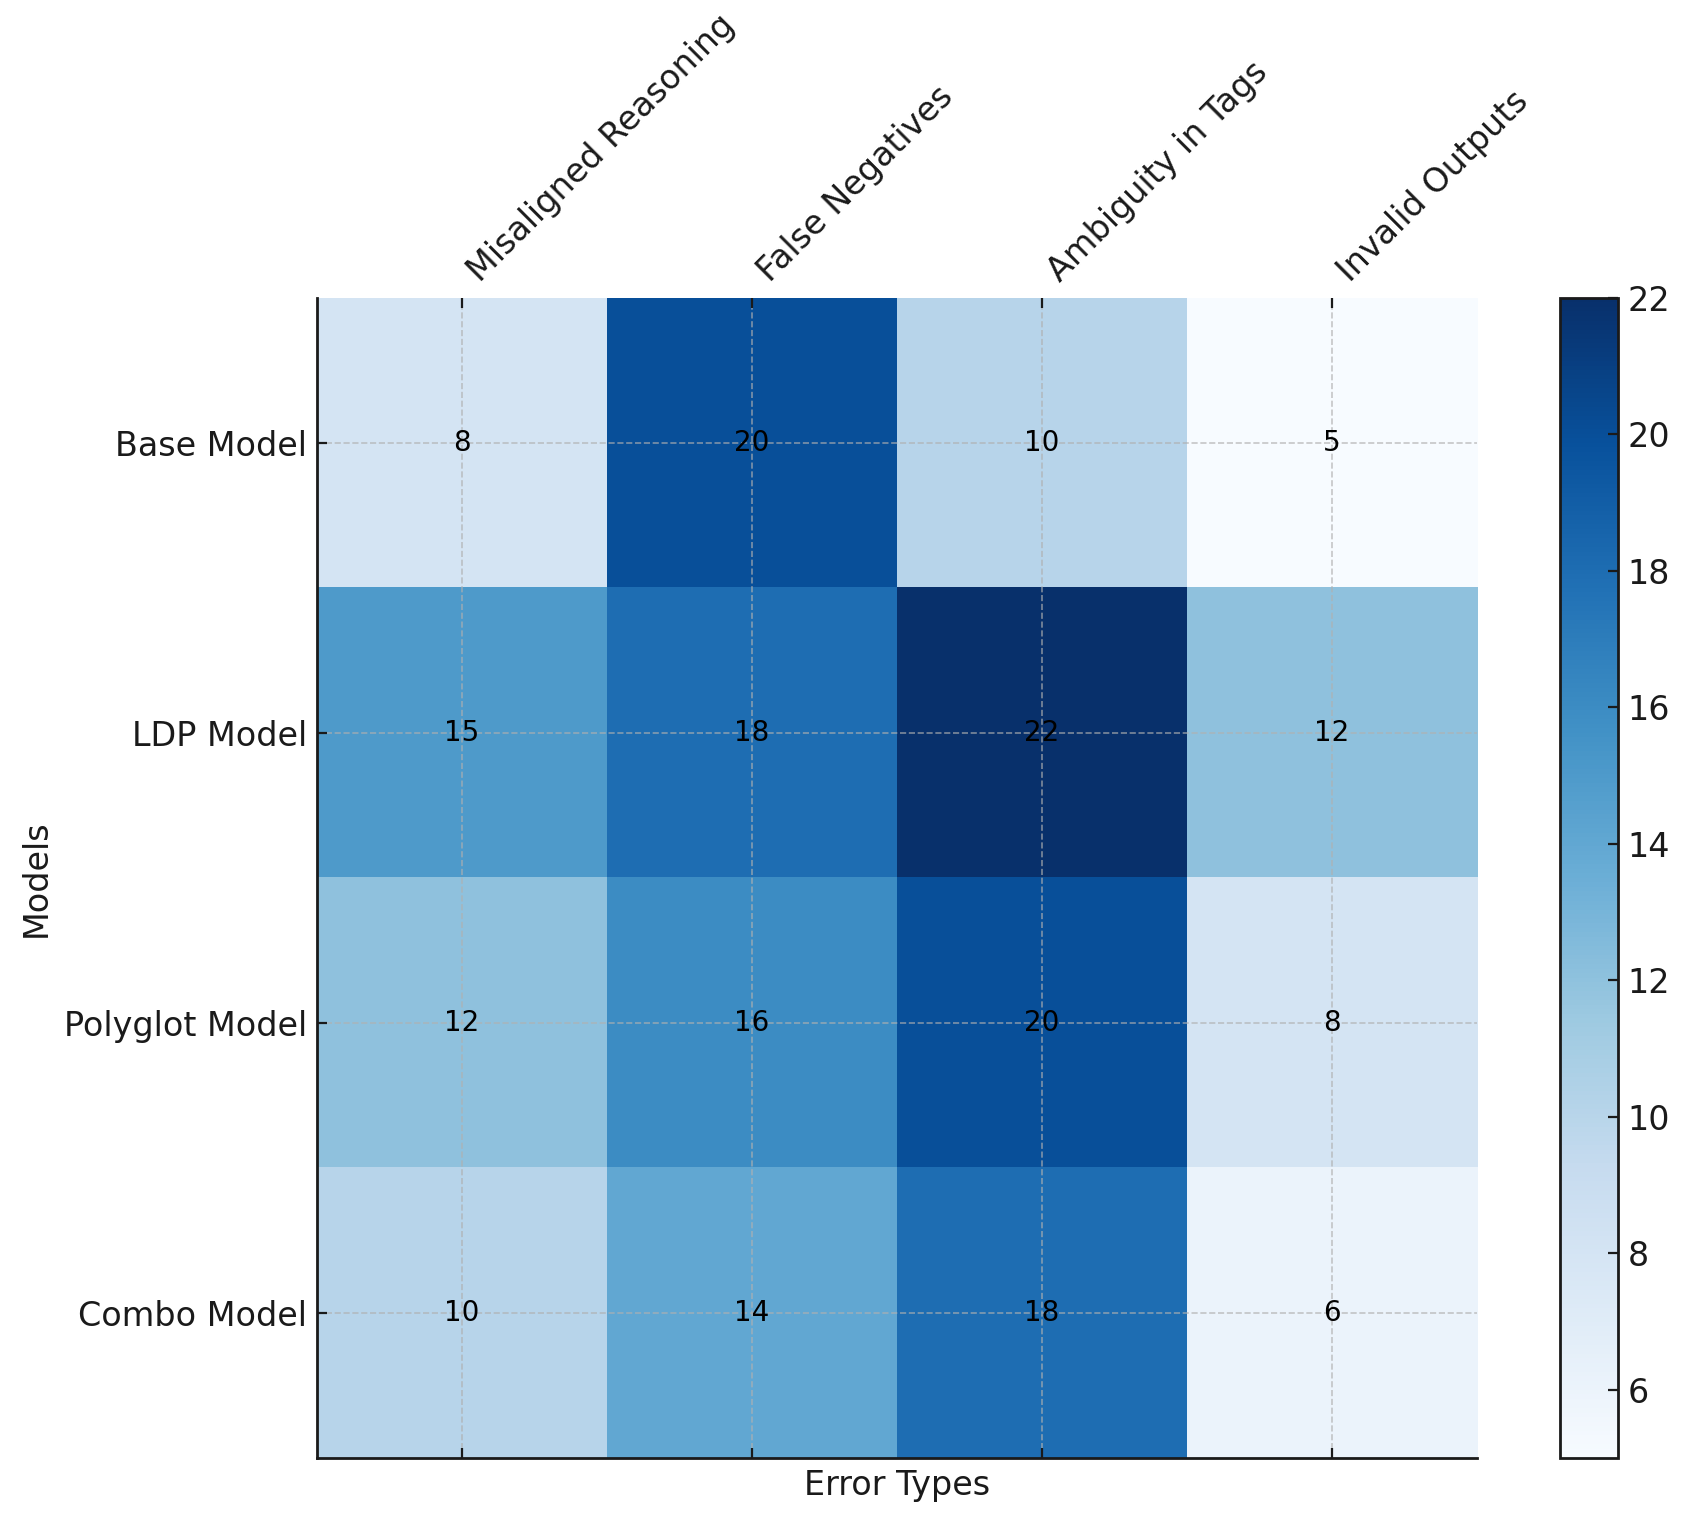
\includegraphics[width= \linewidth]{output.png}
    \caption{NLI Task Confusion Matrix}
    \label{fig:enter-label}
\end{figure}

\paragraph{Errors in Evaluation Metrics:}
During evaluation, certain entries produced blank or invalid values for metrics such as NLI F1, MT BLEU, or MRC F1. These errors often stemmed from the model's inability to distinguish tags for prompts with ambiguous phrasing, low-resource dialectal expressions, or complex linguistic structures. Additionally, evaluation metrics reliant on lexical overlap or strict logical alignment failed to capture meaningful outputs when models deviated significantly from expected formats.

\subsubsection{Table of Errors and Outputs}
Table~\ref{tab:error-analysis} provides examples of errors observed across models. Each row includes an input prompt, the generated output, the expected output, and the specific type of error identified. These examples illustrate the challenges in maintaining linguistic precision, cultural context, and idiomatic meaning.


\subsection{Discussion}
The results underscore the importance of task-specific adaptations in low-resource language processing. While NLI tasks benefit from simpler, generalizable models, MRC and MT tasks require more nuanced approaches that incorporate cultural, poly-glottal data, and conversational context. However, there are some key limitations we identified. 



\subsubsection{Limitations in Dataset Diversity}
A significant limitation lies in the diversity and coverage of the training datasets. Low-resource dialects, such as Haitian Creole and African American Vernacular English (AAVE), are underrepresented, leading to challenges in accurately capturing dialect-specific features. The lack of sufficient examples for dialect mixing and code-switching further exacerbates this issue, as evidenced by frequent misclassification and blending of linguistic features in the models' outputs.

\subsubsection{Limitations in Evaluation Metrics}
The reliance on standard evaluation metrics, such as F1 for NLI and MRC or BLEU for MT, introduces additional limitations. These metrics often fail to account for unconventional but valid outputs, particularly in low-resource language contexts. For instance, the BLEU scores for the MT task were notably low across all models with extreme standard deviations Figure~\ref{fig:mt-analysis}, even for the \textbf{Hybrid Model}, which achieved the highest score. This raises questions about whether BLEU effectively captures the quality of translations in cross-lingual and culturally nuanced scenarios, and if our BLEU scores are a proper indication of translation readability on a basic level. Similarly, blank or invalid metric values highlight the need for evaluation frameworks that can handle ambiguous phrasing and complex linguistic structures more effectively. Perhaps a model fine-tuned on the utilized low-resource language might yield significantly better translation scores while maintaining a similar trend of performance improvement across our four model structures.


\subsubsection{Future Direction}
We believe future work should focus on fine-tuning our model on multiple low-resource languages, as this might further improve translational and comprehension tasks in our combined model. Fine-tuning our model on Natural Language Inference Tasks would also prove to be useful in further studies, as we can then eliminate the disparity found in more complex models when carrying out logical tasks. 
Further testing should be done in other languages and there dialectal variations or similar tongues. For example, Basque and Spanish are both Latin-based languages but not dialects of each other. By including a dialect such Andalusian Spanish, we might be able to yield more results indicating that the \textbf{Hybrid Model} works in a broader cross-lingual context. 
Additionally, we aim to explore speech-to-speech transformations, allowing models to seamlessly process spoken inputs and generate accurate spoken outputs with nuanced responses that honor cultural and contextual cues.










\section{Conclusion}

This study explores low-resource language processing and dialect adaptation in Haitian Creole, focusing on combining Linguistically Diverse Prompting (LDP) and Polyglot Prompting techniques with contextual markers. Our Hybrid Model achieved an F1 score of 0.924 in Machine Reading Comprehension and a BLEU score of 18.057 in Machine Translation in Haitian Creole. While the BLEU score indicates room for improvement, particularly with similar low-resource languages, our findings show that complex models excel in comprehension and translation but under-perform in Natural Language Inference tasks, where simpler models are more consistent.

We introduced a novel approach building on LDP and Polyglot Prompting to adapt models for dialectal variations, analyzing AAVE and Haitian Creole. Error analysis revealed challenges with linguistic ambiguity and code-switching in the tagging, providing insights on improving linguistic and dialectal tagging.

Future work includes expanding to other low-resource languages tested in other studies \cite{Faisal:24} \cite{Nguyen:24} \cite{Ng:22}, observing cross-lingual tasks with audio datasets for low-resource languages, refining evaluation metrics for translation quality, and fine-tuning models to enhance Natural Language Inference performance while maintaining translation and comprehension quality. By testing the broader applicability of our hybridization technique, we can expand the inclusion of other under-developed countries using LLMs.
\section*{Acknowledgments}

\bibliography{custom}
\cleardoublepage
\appendix
\section{Score Figures}
\label{sec:appendix}

\subsection{Natural Language Inference}

\begin{figure}[H]
    \centering
    \includegraphics[width=1\linewidth]{Screenshot 2024-11-25 at 1.36.10 PM.png}
    \caption{Average NLI F1 Score}
    \label{fig:nli-scores}
\end{figure}

\subsection{Machine Reading Comprehension}

\begin{figure}[H]
    \centering
    \includegraphics[width=1\linewidth]{Screenshot 2024-11-25 at 1.35.51 PM.png}
    \caption{Average MRC F1 Score}
    \label{fig:mrc-scores}
\end{figure}

\subsection{Machine Translation}

\begin{figure}[H]
    \centering
    \includegraphics[width=1\linewidth]{Screenshot 2024-11-25 at 1.35.37 PM.png}
    \caption{Average MT BLEU Score}
    \label{fig:mt-scores}
\end{figure}

\section{Prompts}

\subsection{Example Base Model Prompt}\\

\begin{enumerate}
    \item Observe the linguistic features of each entry of \{\textbf{D2}\}.
    \item Translate the entry into Haitian Creole and perform a linguistic analysis on the translation.
    \item Provide the cultural and conversational context of the translation.
    \item Provide a dialogue response in Haitian Creole.
\end{enumerate}\\

\subsection{Example LDP Model Prompt}\\

\begin{enumerate}
    \item Observe the linguistic features in \{\textbf{D2}\}.
    \item Translate the content of each \{\textbf{D2}\} entry into the language or dialect used in its corresponding \{\textbf{D1}\} entry.
    \item Provide a dialogue response or continuation that reflects the content and context of the \{\textbf{D1}\} entry while retaining the tone of \{\textbf{D2}\}.
    \item Ensure consistency with \{\textbf{D1}\}'s language and dialect style across all responses.
    \item Perform a cultural and conversational context analysis of \{\textbf{D1}\} based on \{\textbf{D2}\}.
    \item Provide a dialogue response in language \{\textbf{D1}\} (Haitian Creole) or a continuation based on what the speaker said in language \{\textbf{D2}\} (English).
\end{enumerate}\\

\subsection{Example PolyP Model Prompt}\\

\begin{enumerate}
    \item Conduct a translation task where you translate the dialect in \{\textbf{D1}\} to the dialect/language in \{\textbf{D3}\}.
    \item Perform a cultural and conversational context analysis of \{\textbf{D1}\} based on the shared tags with \{\textbf{D3}\} and report them.
    \item Provide a dialogue response in language \{\textbf{D1}\} or a continuation based on what the speaker said in \{\textbf{D3}\}.
    \item Re-prompt yourself with the same tasks using the language spoken in \{\textbf{D1}\}.
    \item Provide a dialogue response in language \{\textbf{D1}\} (Haitian Creole) or a continuation based on what the speaker said in language \{\textbf{D3}\} (AAVE).
\end{enumerate}\\

\section{Error Analysis}

\subsection{Natural Language Inference}

\begin{figure}[h]
    \centering
    \includegraphics[width=1\linewidth]{Screenshot 2024-12-12 at 6.22.36 PM.png}
    \caption{NLI Bin Analysis}
    \label{fig:enter-label}
\end{figure}

\subsection{Machine Reading Comprehension}

\begin{figure}[h]
    \centering
    \includegraphics[width=1\linewidth]{Screenshot 2024-12-12 at 6.21.56 PM.png}
    \caption{MRC Bin Analysis}
    \label{fig:enter-label}
\end{figure}

\subsection{Machine Translation}

\begin{figure}[h]
    \centering
    \includegraphics[width=1\linewidth]{Screenshot 2024-12-12 at 6.21.33 PM.png}
    \caption{MT Bin Analysis}
    \label{fig:enter-label}
\end{figure}

\clearpage

\subsection{Response Table}

\begin{table}[h] 
\centering
\renewcommand{\arraystretch}{1.4} 
\setlength{\tabcolsep}{5pt} 
\resizebox{\textwidth}{!}{%
\begin{tabular}{|c|p{4cm}|p{4.5cm}|p{4.5cm}|p{3.5cm}|}
\hline
\textbf{Model} & \textbf{Prompt} & \textbf{Model Output} & \textbf{Expected Output} & \textbf{Error Type} \\ \hline
\textbf{Base Model} 
& Translate: Sa k ap fèt? 
& What’s happening? 
& What’s going on? 
& Ambiguity in linguistic tags \\ \hline
\textbf{LDP Model} 
& Provide a formal response to: Yo, what’s good? 
& Hello, how are you? 
& Greetings, how can I assist you? 
& Misaligned reasoning \\ \hline
\textbf{Polyglot Model} 
& Explain this proverb: What goes around, comes around. 
& It’s a cycle. 
& Actions have consequences. 
& Idiomatic challenge \\ \hline
\textbf{Combined Model} 
& Rephrase: I ain’t got nothing. 
& I don’t have anything. 
& I do not have anything. 
& False negatives \\ \hline
\end{tabular}%
}
\caption{Examples of errors observed in responses.}
\label{tab:error-analysis}
\end{table}







\end{document}
